\begin{frame}

\begin{center}
  \usebeamerfont*{title} \usebeamercolor[fg]{title} \huge Analisi dei requisiti
\end{center}

\end{frame}

\section{Analisi dei requisiti}
\begin{frame}
  \frametitle{Scopo del progetto}

  \begin{center}
    Convertire MaaP in un servizio ed ampliare le funzionalità offerte agli utenti.
  \end{center}
\end{frame}

\begin{frame}
  \frametitle{Cos'è MaaP?}

  MaaP è un applicazione web destinata alle aziende, che permette di creare delle interfacce HTML per la visualizzazione di dati aziendali.

   \includegraphics[width=0.6\columnwidth]{HomeMaap.png}
  
\end{frame}

\begin{frame}
  \frametitle{Requisiti Principali}

  \begin{itemize}
  \item Un utente deve poter iscrivere la propria azienda;
  \item Il proprietario dell'azienda può invitare dei collaboratori;
  \item Un utente può collegare la sua base di dati al servizio;
  \item Tramite un editor deve essere possibile creare delle viste per i propri dati;
  \item Deve essere accessibile la visualizzazione dei propri dati tramite le viste create.
  \end{itemize}
\end{frame}


\begin{frame}
  \frametitle{Utenti del sistema}

  \begin{itemize}
  \item \textbf{Super-Admin}: proprietario del servizio
  \item \textbf{Owner}: proprietario di una Company
  \item \textbf{Admin}: amministratore di una Company
  \item \textbf{Member}: utente registrato, dipendente di una Company
  \item \textbf{Guest}: utente temporaneo di una Company
  \end{itemize}

\end{frame}

\begin{frame}
  \frametitle{Utenti del sistema}
  Il Super-Admin deve poter:
  \begin{columns}
    \begin{column}{0.5\textwidth}   
    \begin{itemize}
    \item Creare delle nuove Companies;
    \item Gestire le Companies esistenti;
    \item Gestire gli utenti esistenti;
    \item Aggiungere nuovi Super-Admin.
    \end{itemize}
    \end{column}
    \begin{column}{0.5\textwidth}
    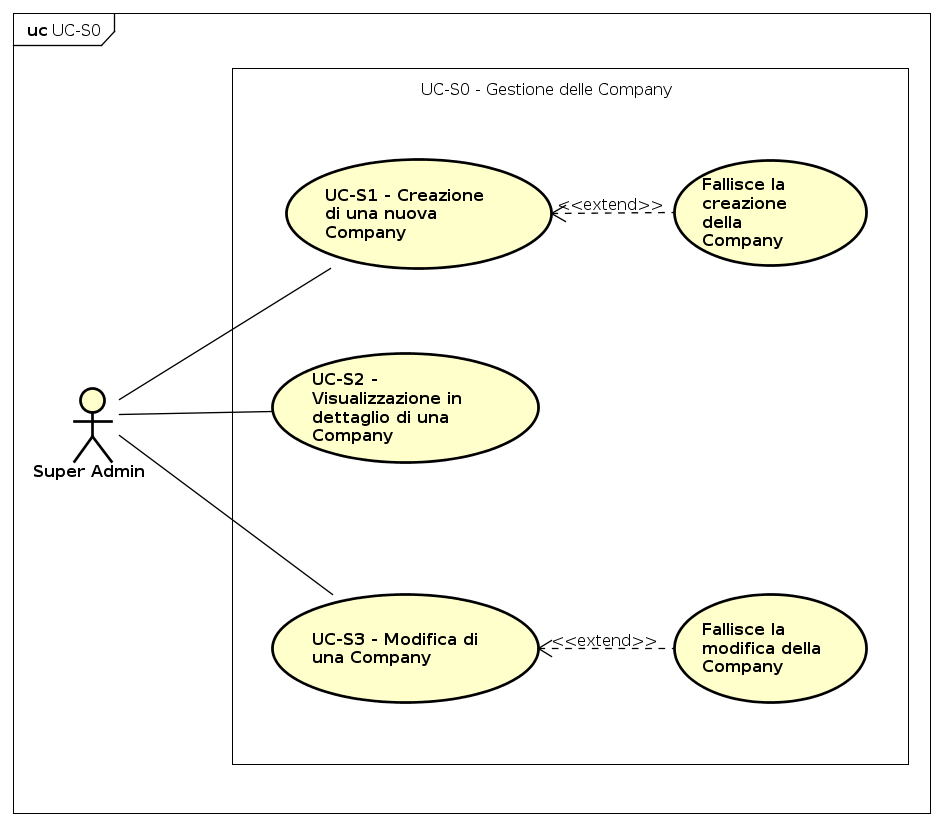
\includegraphics[width=0.9\columnwidth]{SuperAdmin.png}
    \end{column}
  \end{columns}
\end{frame}

\begin{frame}
  \frametitle{Utenti del sistema}
  Owner, Admin e Member possono:
  \begin{columns}
    \begin{column}{0.5\textwidth}
       \begin{itemize}
       \item Creare nuove viste utilizzando l'editor;
       \item Visualizzare e disporre le viste nella propria dashboard utente.
       \end{itemize}
    \end{column}
    \begin{column}{0.5\textwidth}
    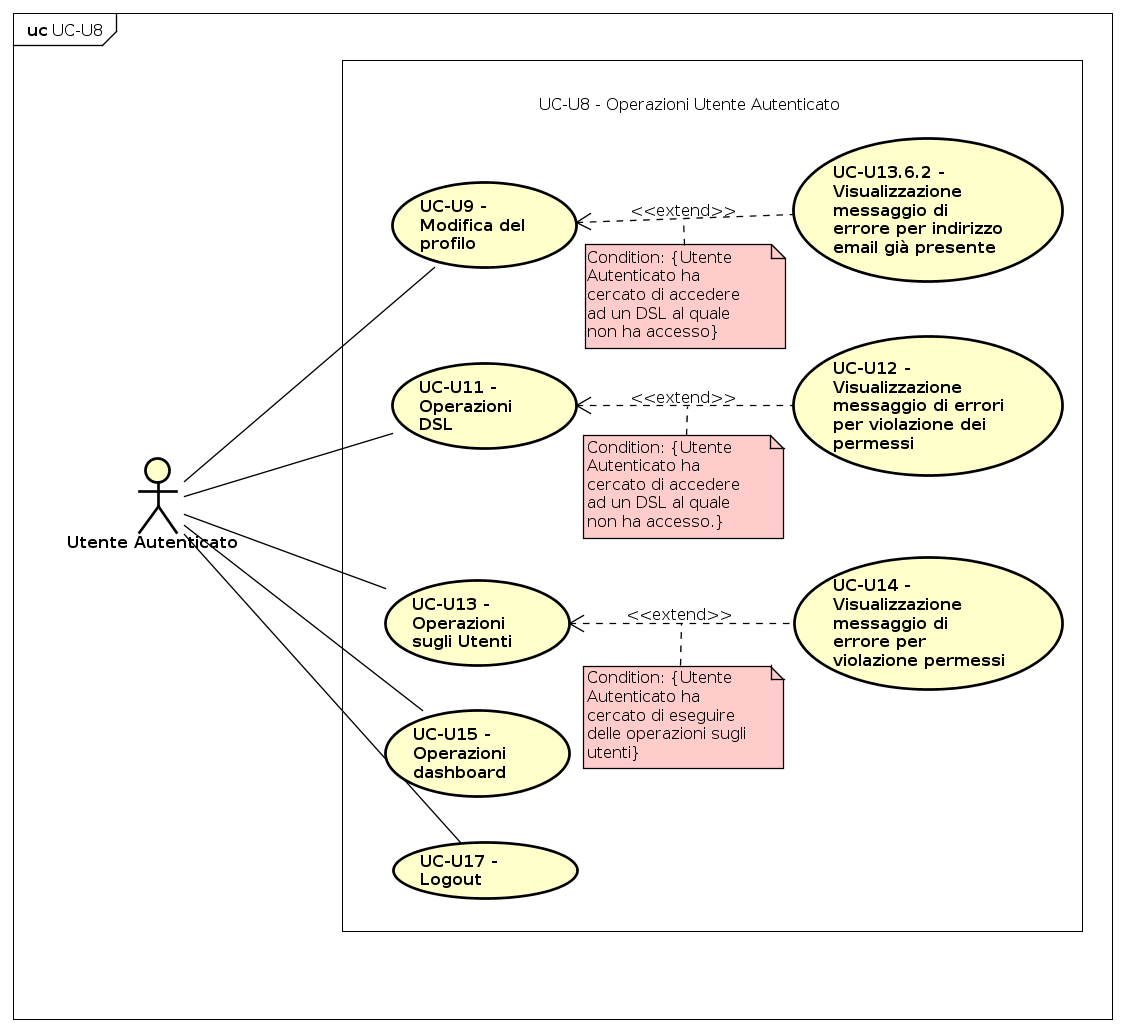
\includegraphics[width=0.9\columnwidth]{UCUtenti.png}
    \end{column}
  \end{columns}
\end{frame}

\begin{frame}
  \frametitle{Utenti del sistema}
  Inoltre:
  \begin{itemize}
  \item L'Owner può concedere e revocare privilegi di admin;
  \item L'Admin e l'Owner possono gestire gli utenti della Company.
  \end{itemize}

\end{frame}

\begin{frame}
  \frametitle{L'editor}
  \begin{columns}
    \begin{column}{0.5\textwidth}
      \begin{itemize}
      \item Permette di creare intuitivamente le viste per gli utenti;
      \item Deve permettere di esportare i dati in formati Json e CSV;
      \item Deve dare la possibilità di modifica agevole delle viste.
      \end{itemize}
    \end{column}
    \begin{column}{0.7\textwidth}
    	\centering
       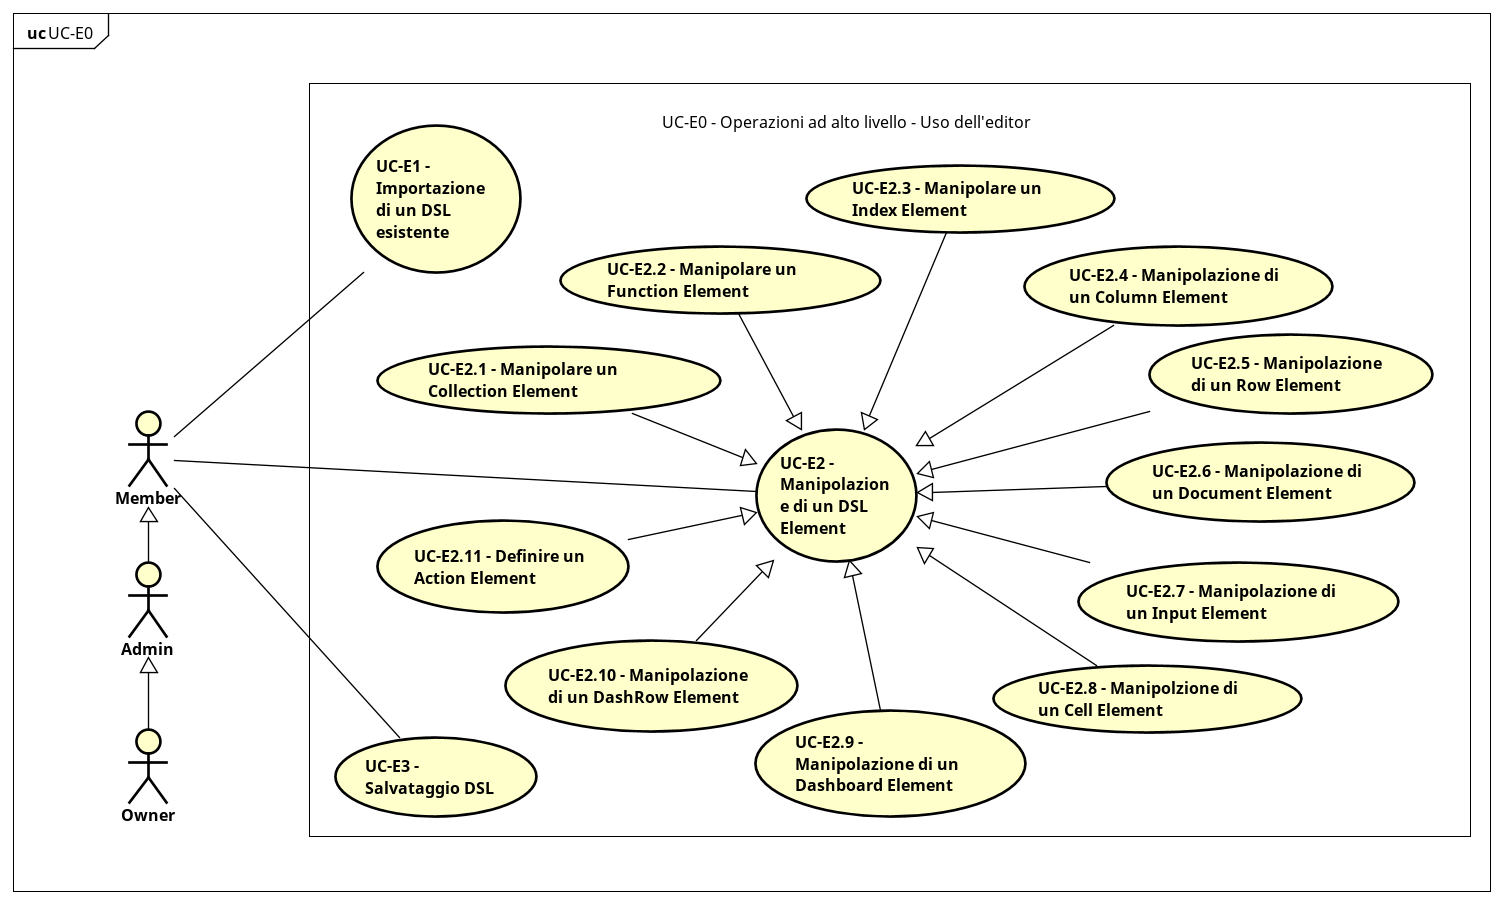
\includegraphics[width=0.9\columnwidth]{Editor.png}
    \end{column}
  \end{columns}
  
\end{frame}

\section{Piano di Progetto}
\begin{frame}
\begin{center}
  \usebeamerfont*{title} \usebeamercolor[fg]{title} \huge Piano di Progetto
\end{center}
\end{frame}

\begin{frame}
  \frametitle{Modello di ciclo di vita scelto}

  \begin{columns}
    \begin{column}{0.6\textwidth}
      
      Il modello di ciclo di vita scelto è quello \textbf{incrementale} perchè:
      \begin{itemize}
      \item Permette di monitorare l'evoluzione del progetto;
      \item Si ottiene una base verificata alla fine di ogni processo;
      \item Permette l'alternanza tra le attività.
      \end{itemize}
    \end{column}
    \begin{column}{0.4\textwidth}
      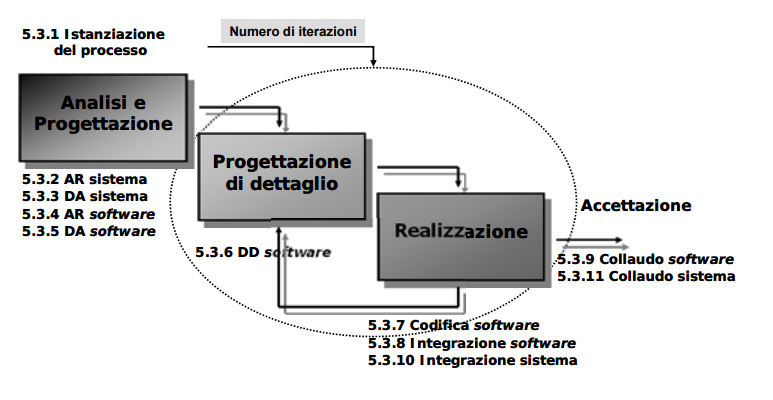
\includegraphics[width=0.9\columnwidth]{Incrementale.png}
    \end{column}
  \end{columns}
\end{frame}


\begin{frame}
  \frametitle{Rischi individuati}
  Per una migliore organizzazione sono stati suddivisi per tipologie:
  \begin{itemize}
  \item Tecnologici;
  \item Derivanti dalle persone;
  \item Organizzativi;
  \item Derivanti dal software;
  \item Derivanti dai requisiti;
  \item Derivanti da stime errate.
  \end{itemize}
\end{frame}
  
\begin{frame}
    \frametitle{Rischi individuati - Derivanti dalle persone}

    Sono i rischi con probabilità maggiore. In particolare sono stati individuati rischi riguardanti:
    \begin{columns}
      \begin{column}{0.5\textwidth}
        \begin{itemize}
        \item La disponibilità di tempo dei membri del gruppo;
        \item La possibilità di conflitti tra elementi del gruppo;
        \item Le lacune portate dalla poca conoscenza delle tecnologie applicate.
        \end{itemize}
      \end{column}
      \begin{column}{0.5\textwidth}
        
\includegraphics[width=0.8\columnwidth]{focus_group}
      \end{column}
    \end{columns}
\end{frame}

\begin{frame}
  \frametitle{Rischi individuati - Rischi sul software}
  \begin{columns}
    \begin{column}{0.5\textwidth}
  Rischi che derivano dal software utilizzato per sviluppare il progetto.\\
  Il rischio di indisposizione delle piattaforme Teamwork e GitHub su cui si appoggia il progetto, seppur la probabilità di verificarsi sia remota, porterebbe disagi notevoli per il progetto.
    \end{column}
    \begin{column}{0.5\textwidth}
      
\includegraphics[width=0.6\columnwidth]{github.png}\\
      
\includegraphics[width=0.6\columnwidth]{teamwork.png}
    \end{column}
  \end{columns}
\end{frame}

\begin{frame}
  \frametitle{Rischi individuati - Derivanti dai requisiti}
    Punto di rischio con maggior impatto e probabilità per il progetto.
    I rischi sono dovuti a:
    \begin{itemize}
    \item Comprensione errata dei requisiti;
    \item Cambiamento di alcuni dei requisiti individuati.
    \end{itemize}    
\end{frame}

\begin{frame}
  \frametitle{Pianificazione del progetto}
  Seguirà la seguente ripartizione delle ore:
  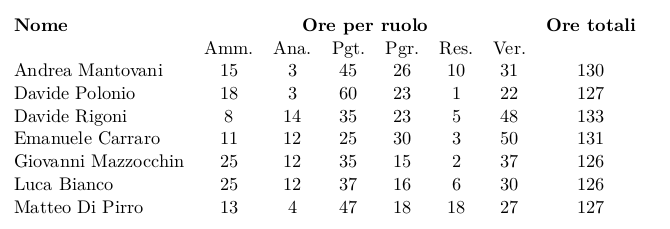
\includegraphics[width=0.6\textwidth]{RipartizioneOre.png}
  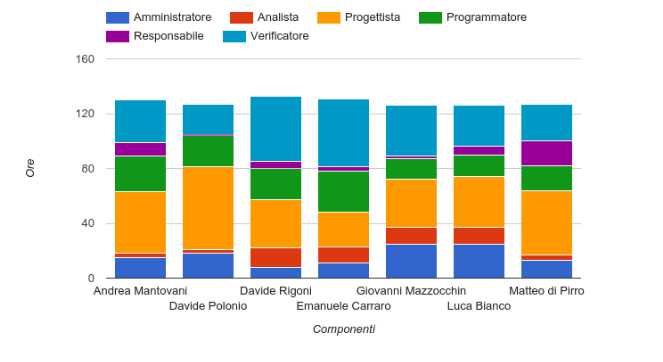
\includegraphics[width=0.5\textwidth]{RipOreGrafico.png}

\end{frame}

\begin{frame}
  \frametitle{Preventivo calcolato}
  Per la realizzazione dell'intero progetto si è preventivato quanto segue:

  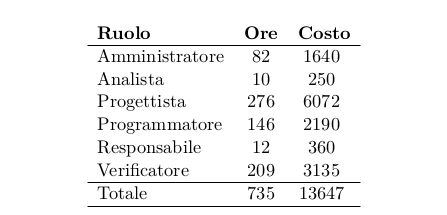
\includegraphics[width=0.5\textwidth]{TabCosti.png}
  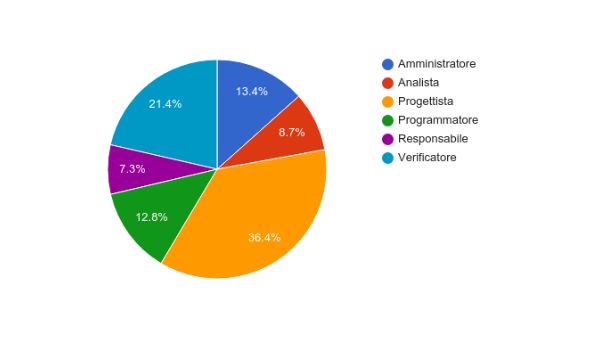
\includegraphics[width=0.5\textwidth]{CostoRipartizione.png}
\end{frame}


